\begin{figure}[htbp]
			\centering
			\resizebox{\textwidth}{!}{%
				\begin{tikzpicture}[
					scale=0.95,
					>=latex,
					trave/.style={line width=1.4pt},
					carico/.style={black, line width=0.6pt},
					forza/.style={black, line width=0.8pt},
					diagT/.style={black, line width=0.6pt},
					diagM/.style={black, line width=0.6pt},
					hatch/.style={gray!50, line width=0.3pt},
					quota/.style={black, line width=0.4pt},
					fibre/.style={gray!70, line width=0.3pt},
					]
					
					% ── Parametri dei vincoli (convenzione C06/C07) ──
					\def\tw{0.15}    \def\thR{0.28}   \def\rn{0.06}
					\def\rw{0.05}    \def\bw{0.09}    \def\gw{0.22}
					\def\hh{0.10}
					
					% ── Geometria del problema ──
					\def\Lell{4}                            % lunghezza trave ℓ
					\pgfmathsetmacro{\xA}{0}
					\pgfmathsetmacro{\xMid}{0.5*\Lell}      % mezzeria

					\pgfmathsetmacro{\xZstar}{\Lell/3}
					\def\yqi{-0.80}                         % y delle quote sotto la trave
					\def\ylab{-3.30}                        % y delle etichette di pannello
					
					% ── Parametri del simbolo "coppia concentrata" ──
					\def\rCoppia{0.25}    % raggio dell'arco
					\def\Lwing{0.08}      % lunghezza dell'ala della freccia
					
					% =========================================================
					% PANNELLO (a) — Schema statico
					% =========================================================
					\begin{scope}[xshift=0cm]
						
						% ── Trave ──
						\draw[trave] (0,0) -- (\Lell,0);
						
						% ── Fibra inferiore (tratteggio sotto la trave) ──
						\draw[fibre, dashed] (0, -0.1) -- (\Lell, -0.1);
						
						% ── Cerniera in A ──
						\draw[thick] (0,0) -- (-\tw,-\thR) -- (\tw,-\thR) -- cycle;
						\draw[thick] (-\gw,-\thR) -- (\gw,-\thR);
						\foreach \x in {-0.16,-0.08,0,0.08,0.16}
						\draw[thin] (\x,-\thR) -- ++(-0.07,-\hh);
						
						% ── Carrello verticale in B ──
						\draw[thick] (\Lell,0) -- (\Lell-\tw,-\thR) -- (\Lell+\tw,-\thR) -- cycle;
						\draw[thick] (\Lell-\bw,-\thR-\rw-0.01) circle (\rw);
						\draw[thick] (\Lell+\bw,-\thR-\rw-0.01) circle (\rw);
						\draw[thick] (\Lell-\gw,-\thR-2*\rw-0.04) -- (\Lell+\gw,-\thR-2*\rw-0.04);
						\foreach \x in {-0.16,-0.08,0,0.08,0.16}
						\draw[thin] (\Lell+\x,-\thR-2*\rw-0.04) -- ++(-0.07,-\hh);
						
						% ── Anellini bianchi sui perni ──
						\draw[thick, fill=white] (0,0) circle (\rn);
						\draw[thick, fill=white] (\Lell,0) circle (\rn);
						
						% ── Etichette A, B (ancorate sotto, perché sopra c'è la coppia) ──
						\node[above left=-2pt,  font=\small] at (0,0)      {$A$};
						\node[above right=-2pt, font=\small] at (\Lell,0)  {$B$};
						
						% ── Parametri del simbolo "coppia concentrata" ──
						\def\rCoppia{0.25}    % raggio dell'arco
						\def\Lwing{0.12}      % lunghezza dell'ala della freccia (era 0.08)
						
						\def\AoffX{0.20}    % offset orizzontale del semicerchio di μ_A (verso destra)
						\def\BoffX{0.20}    % offset orizzontale del semicerchio di μ_B (verso sinistra)
						
						% ── Coppia antioraria in A: semicerchio sul lato DESTRO che attraversa la trave ──
						\draw[forza](\AoffX, -\rCoppia)
						arc[start angle=-90, end angle=90, radius=\rCoppia];
						% Punta della freccia all'estremità superiore (a +90°): punta verso sinistra
						\pgfmathsetmacro{\tipxA}{\AoffX}
						\pgfmathsetmacro{\tipyA}{\rCoppia}
						\draw[forza] (\tipxA, \tipyA)
						-- ({\tipxA + \Lwing*cos(25)},  {\tipyA + \Lwing*sin(25)});
						\draw[forza] (\tipxA, \tipyA)
						-- ({\tipxA + \Lwing*cos(-25)}, {\tipyA + \Lwing*sin(-25)});
						\node[right, font=\footnotesize] at ({\AoffX-\rCoppia+0.3}, 0.3) {$\mu_A$};
						
						
						% ── Coppia antioraria in B: semicerchio sul lato SINISTRO che attraversa la trave ──
						\draw[forza](\Lell-\BoffX, \rCoppia)
						arc[start angle=90, end angle=270, radius=\rCoppia];
						\pgfmathsetmacro{\tipxB}{\Lell-\BoffX}
						\pgfmathsetmacro{\tipyB}{-\rCoppia}
						\draw[forza] (\tipxB, \tipyB)
						-- ({\tipxB + \Lwing*cos(155)}, {\tipyB + \Lwing*sin(155)});
						\draw[forza] (\tipxB, \tipyB)
						-- ({\tipxB + \Lwing*cos(205)}, {\tipyB + \Lwing*sin(205)});
						\node[left, font=\footnotesize] at ({\Lell-\BoffX+\rCoppia-0.3}, 0.3) {$\mu_B$};
						
						
						% ── Quota ℓ sotto la trave ──
						\draw[<->, quota] (0,\yqi) -- (\Lell,\yqi);
						\draw[quota] (0,\yqi+0.07)     -- (0,\yqi-0.07);
						\draw[quota] (\Lell,\yqi+0.07) -- (\Lell,\yqi-0.07);
						\node[above, font=\small] at (\xMid, \yqi-0.04) {$\ell$};
						
						% Etichetta pannello (a)
						\node[font=\small] at (0.5*\Lell, 0.4*\ylab) {(a)};
						
					\end{scope}
					
					% =========================================================
					% PANNELLO (b) — Diagramma di T(z)
					% =========================================================
					\begin{scope}[xshift=5.5cm]
						
						% ── Trave (clone) ──
						\draw[trave] (0,0) -- (\Lell,0);
						
						% ── Vincoli (clone) ──
						\draw[thick] (0,0) -- (-\tw,-\thR) -- (\tw,-\thR) -- cycle;
						\draw[thick] (-\gw,-\thR) -- (\gw,-\thR);
						\foreach \x in {-0.16,-0.08,0,0.08,0.16}
						\draw[thin] (\x,-\thR) -- ++(-0.07,-\hh);
						\draw[thick] (\Lell,0) -- (\Lell-\tw,-\thR) -- (\Lell+\tw,-\thR) -- cycle;
						\draw[thick] (\Lell-\bw,-\thR-\rw-0.01) circle (\rw);
						\draw[thick] (\Lell+\bw,-\thR-\rw-0.01) circle (\rw);
						\draw[thick] (\Lell-\gw,-\thR-2*\rw-0.04) -- (\Lell+\gw,-\thR-2*\rw-0.04);
						\foreach \x in {-0.16,-0.08,0,0.08,0.16}
						\draw[thin] (\Lell+\x,-\thR-2*\rw-0.04) -- ++(-0.07,-\hh);
						\draw[thick, fill=white] (0,0) circle (\rn);
						\draw[thick, fill=white] (\Lell,0) circle (\rn);
						
						% ── Etichette A, B ──
						\node[above left=-2pt,  font=\small] at (0,0)      {$A$};
						\node[above right=-2pt, font=\small] at (\Lell,0)  {$B$};
						
						% ── Diagramma T(z) ──   QUI HO FATTO CASINO!!!!
						\def\sT{0.67}
						\pgfmathsetmacro{\Tval}{(3/\Lell)*\sT}    % T(z) = 3/ℓ → 0.75·0.67 ≈ 0.50
						
						% Hatching verticale uniforme su tutta la trave
						\foreach \x in {0.10, 0.30, ..., 3.90} {
							\draw[hatch] (\x, 0) -- (\x, \Tval);
						}
						
						% Bordo del diagramma — rettangolo
						\draw[diagT]
						(0, 0) -- (0, \Tval)             % verticale in A
						-- (\Lell, \Tval)                % uniforme su tutta la trave
						-- (\Lell, 0);                   % verticale di chiusura in B
						
						% Segno cerchiato al centro del rettangolo
						\node[font=\small] at (\xMid, {0.5*\Tval})	{$\boldsymbol{\oplus}$};
						
						% Etichetta del valore (μ_A+μ_B)/ℓ sopra il rettangolo, a destra
						\node[above, font=\small] at (\Lell-0.3, \Tval)	{$\tfrac{\mu_A + \mu_B}{\ell}$};
						
						% Etichetta pannello (b)
						\node[font=\small] at (0.5*\Lell, 0.4*\ylab) {(b)};
						
					\end{scope}
					
					% =========================================================
					% PANNELLO (c) — Diagramma di M(z)
					% =========================================================
					\begin{scope}[xshift=11.0cm]
						
						% ── Trave (clone) ──
						\draw[trave] (0,0) -- (\Lell,0);
						
						% ── Vincoli (clone) ──
						\draw[thick] (0,0) -- (-\tw,-\thR) -- (\tw,-\thR) -- cycle;
						\draw[thick] (-\gw,-\thR) -- (\gw,-\thR);
						\foreach \x in {-0.16,-0.08,0,0.08,0.16}
						\draw[thin] (\x,-\thR) -- ++(-0.07,-\hh);
						\draw[thick] (\Lell,0) -- (\Lell-\tw,-\thR) -- (\Lell+\tw,-\thR) -- cycle;
						\draw[thick] (\Lell-\bw,-\thR-\rw-0.01) circle (\rw);
						\draw[thick] (\Lell+\bw,-\thR-\rw-0.01) circle (\rw);
						\draw[thick] (\Lell-\gw,-\thR-2*\rw-0.04) -- (\Lell+\gw,-\thR-2*\rw-0.04);
						\foreach \x in {-0.16,-0.08,0,0.08,0.16}
						\draw[thin] (\Lell+\x,-\thR-2*\rw-0.04) -- ++(-0.07,-\hh);
						\draw[thick, fill=white] (0,0) circle (\rn);
						\draw[thick, fill=white] (\Lell,0) circle (\rn);
						
						% ── Etichette A, B ──
						\node[above left=-2pt,  font=\small] at (0,0)      {$A$};
						\node[above right=-2pt, font=\small] at (\Lell,0)  {$B$};
						
						% ── Punto z* dove M=0 ──
						\draw[forza] (\xZstar, -0.10) -- (\xZstar, 0.10);
						
						% ── Diagramma M(z) ──
						\def\sM{0.50}
						\pgfmathsetmacro{\MAfig}{ 1*\sM}      % M(A) = -μ_A = -1 → sopra: +0.40
						\pgfmathsetmacro{\MBfig}{-2*\sM}      % M(B) = +μ_B = +2 → sotto: -0.80
						
						% Hatching tratto [0, z*]: lineare, sopra l'asse (M<0)
						\foreach \x in {0.10, 0.30, ..., 1.30} {
							\pgfmathsetmacro{\h}{\MAfig*(1 - \x/\xZstar)}
							\draw[hatch] (\x, 0) -- (\x, \h);
						}
						% Hatching tratto [z*, ℓ]: lineare, sotto l'asse (M>0)
						\foreach \x in {1.50, 1.70, ..., 3.90} {
							\pgfmathsetmacro{\h}{\MBfig*(\x - \xZstar)/(\Lell - \xZstar)}
							\draw[hatch] (\x, 0) -- (\x, \h);
						}
						
						% Bordo del diagramma — retta da (0, MAfig) a (ℓ, MBfig), con chiusure verticali agli estremi
						\draw[diagM]
						(0, 0) -- (0, \MAfig)            % verticale di chiusura in A
						-- (\Lell, \MBfig)               % retta attraverso lo zero in z*
						-- (\Lell, 0);                   % verticale di chiusura in B
						
						% Etichette dei valori notevoli
						% μ_A: sopra il vertice in A (lobo negativo)
						\node[above, font=\small] at (0, \MAfig+0.04) {$\mu_A$};
						% μ_B: sotto il vertice in B (lobo positivo)
						\node[right, font=\small] at (\Lell, \MBfig-0.04) {$\mu_B$};
						% z* sotto la tacca
						\node[below, font=\footnotesize] at (\xZstar, -0.12) {$z^*$};
						
						% Etichetta pannello (c)
						\node[font=\small] at (0.5*\Lell, 0.4*\ylab) {(c)};
						
					\end{scope}
					
				\end{tikzpicture}
			}
			\caption{Trave appoggiata con coppie concentrate antiorarie
				$\mu_A$ in $A$ e $\mu_B$ in $B$:
				(a)~schema strutturale;
				(b)~diagramma del taglio $T(z)$, uniforme pari a
				$(\mu_A + \mu_B)/\ell$ su tutta la trave;
				(c)~diagramma del momento flettente $M(z)$, lineare
				crescente da $-\mu_A$ in $A$ a $\mu_B$ in $B$, con
				annullamento in $z^* = \mu_A\ell/(\mu_A+\mu_B)$.}
			\label{fig:stat_trasv_iso_07}
		\end{figure}
